\section{Project implementations}

The project implementation is divided in several sections, where each section
is described. First we've got an overall description of the project which we've
implemented.

\subsection{Overall description}
The Sensor network project we've made consist of a sink and a mote. The
temperature mote has one single timer which is fired with some constant
frequency. When it has received $n$ measurements it send the results to the
sink. This means our temperature mote is only on when not measuring or sensing
and therefore it's using duty cycling. 

Our current implementation has the structure according to figure \ref{fig:overalloverview}.
\begin{figure}[htbp]
   \centering
   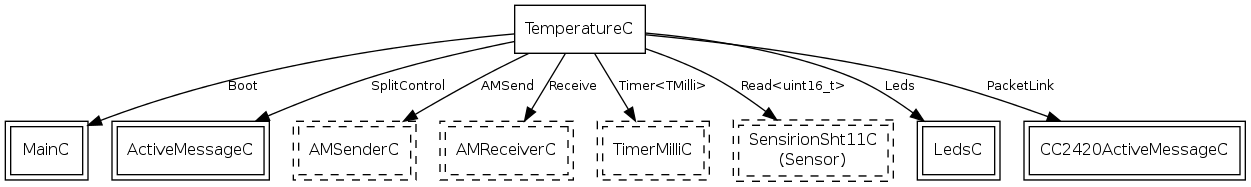
\includegraphics[width=17cm]{img/TemperatureAppC.png} 
   \caption{An overall illustration of the project implmented}
   \label{fig:overalloverview}
\end{figure}

\subsection{Temperature measuring}
Here we'll explain how and where we convert the digital readout from the
temperature sensor to actual degress. The conversion given a digital readout
($SO_{T}$) to a temperature value is given at the following
formula\cite{temperature}:

\begin{align*}
	T &= d_{1} + d_{2} \cdot SO_{T}
\end{align*}
where the coefficients is defined in Table~\ref{table:temperature}.
\begin{table}[ht]
\centering
\begin{tabular}{ | l | c | r | }
	\hline
	VDD & $d_{1} \ ^{\circ}  C$ & $d_{1} \ ^{\circ}  F$ \\
	\hline \hline
	5V & -40.1 & -40.2 \\
	\hline
	4V & -39.8 & -39.6 \\
	\hline
	3.5V & -39.7 & -39.5 \\
	\hline
	3V & -39.6 & -39.3 \\
	\hline
	2.5V & -39.4 & -38.9 \\
	\hline
\end{tabular}
\begin{tabular}{ | l | c | r | }
	\hline
	$SO_{T}$ & $d_{2}  \ ^{\circ}C$ & $d_{2} \ ^{\circ} F$ \\
	\hline \hline
	14 bit & 0.01 & 0.018 \\
	\hline
	12 bit & 0.04 & 0.072\\
	\hline
\end{tabular}
\caption{Temperature conversion coefficients}
\label{table:temperature}
\end{table}
The conversion from a digital readout is being done in the event readDone.
We've made two compile time constants, $CONVERSION_{D1}$, and
$CONVERSION_{D2}$. Both constants are scaled by 100. This allows us to only use
unsigned integers, and recive a more fine-grained temperature measurement.

\begin{lstlisting}[caption={Temperature.h}]
CONVERSION_D1 = 3960, /* VDD = 3V */
CONVERSION_D2 = 1 /* 14 bits */
\end{lstlisting}

\begin{lstlisting}[caption={TemperatureC.nc}]
event void Read.readDone(error_t result, uint16_t data) {
	float tempC;
	if (result != SUCCESS){
		data = 0xffff;
		report_problem();
	}
	// conversion
	tempC = ( (-CONVERSION_D1) + (CONVERSION_D2 * data) ) ;
	reading++;
	average = average + (tempC / NREADINGS);
	if (reading == NREADINGS) {
		local.averages[averages++] = average;
		average = 0;
		reading = 0;
	}
}
\end{lstlisting}

\subsection{Acknowledgement}
In this project one of our goals are to make sure that the motes retransmit the
packages if they do not recive an $ACK$ at the first transmission.

\subsubsection{Package ACK with PacketAcknowledgements interface}

Our first implementation of this involved using the
$tos.interfaces.PacketAcknowledgements$ interface \cite{telosbAPI}. This
interface allows the user to request an acknowledgement on a package before
sending it.

The wireing off the ActiveMessageC PacketAcknowledgements interface onto the
TemperatureC PacketAcknowledgements.

\begin{lstlisting}[caption={TemperatureAppC.nc}]
 TemperatureC.PacketAcknowledgements -> ActiveMessageC;
\end{lstlisting}

We have defined a function in the $TemperatureC.nc$ file that are responsible
for sending the messages. This function requests an acknowledgement on the
message, sends the message and increments the counter responsible for keeping
track on the numbers of times we have tried to transmit a packaged.

\begin{lstlisting}[caption={TemperatureC.nc $\rightarrow$ sendReadings()}]
memcpy(call AMSend.getPayload(&sendBuf, sizeof(local)),
    &local, sizeof local);
call PacketAcknowledgements.requestAck(&sendBuf);
if (call AMSend.send(SINK_NR, &sendBuf, sizeof local) == SUCCESS) {
    sendBusy = TRUE;
    ackTries++;
}
\end{lstlisting}

In the same file we have an event that are trickered when the $send$ is done.
In this function we ask the $PacketAcknowledgements$ interface if the packaged
recived an acknowledgement. If it did, we reset our counter, else we check if
our counter has reached the max number of tries and retransmits the packaged.

\begin{lstlisting}[caption={TemperatureC.nc $\rightarrow$ AMSend.sendDone()}]
if(call PacketAcknowledgements.wasAcked(msg)) {
    reportSent();
    ackTries = 0;
} else {
    if (ackTries < NACKTRIES) {
        sendReadings();
    } else if (ackTries == NACKTRIES) {
        ackTries = 0;
        sleep();
    }
}
\end{lstlisting}

This approach has the disadvantage that the application has to maintain a
secound timer to time the retry delay.

\subsubsection{Package ACK with PacketLink interface}

After more digging in the API we desided to try implementing the package
acknowledgement with the $tos.interfaces.PacketLink$ interface \cite{telosbAPI}.

\begin{lstlisting}[caption={TemperatureAppC.nc}]
TemperatureC.PacketLink -> CC2420ActiveMessageC;
\end{lstlisting}

This part of the implementation looks a lot like the implementation with \\
$tos.interfaces.PacketAcknowledgements$.

\begin{lstlisting}[caption={TemperatureC.nc $\rightarrow$ sendReadings()}]
memcpy(call AMSend.getPayload(&sendBuf, sizeof(local)),
    &local, sizeof local);
call PacketLink.setRetries(&sendBuf, NACKTRIES);
call PacketLink.setRetryDelay(&sendBuf, RETRYDELAY);
if (call AMSend.send(SINK_NR, &sendBuf, sizeof local) == SUCCESS) {
    sendBusy = TRUE;
}
\end{lstlisting}

One of the places where the usage of $PacketLink$ differs from the usage of \\
$PacketAcknowledgements$ is in the $sendDone()$ function. The application does
not have to manually resend the package, but only have to handle the case where
even the retransmits does not get an acknowledgement.

\begin{lstlisting}[caption={TemperatureC.nc $\rightarrow$ AMSend.sendDone()}]
if (call PacketLink.wasDelivered(msg)){
    reportSent();
    sleep();
} else {
    reportProblem();
    sleep();
}
\end{lstlisting}


